\title{バージョン管理システムチュートリアル}

\begin{document}

\begin{frame}
  \titlepage
\end{frame}

\section*{Outline}
\begin{frame}
  \tableofcontents
\end{frame}

\section{チュートリアルの概要}

\begin{frame}{ALPSチュートリアル スタッフ}
  \begin{itemize}
  \item 講師
    \begin{itemize}
    \item 藤堂眞治 (東大物性研) \ \href{mailto:wistaria@issp.u-tokyo.ac.jp}{wistaria@issp.u-tokyo.ac.jp}
    \item 五十嵐 亮 (東大物性研) \ \href{mailto:rigarash@issp.u-tokyo.ac.jp}{rigarash@issp.u-tokyo.ac.jp}
    \item 松尾春彦 (RIST) \ \href{mailto:halm@rist.or.jp}{halm@rist.or.jp}
    \item 本山裕一 (東大院工) \ \href{mailto:yomichi@looper.t.u-tokyo.ac.jp}{yomichi@looper.t.u-tokyo.ac.jp}
    \end{itemize}
  \item 主催
    \begin{itemize}
    \item CMSI: 計算物質科学イニシアティブ \url{http://cms-initiative.jp/}
    \end{itemize}
  \item 共催
    \begin{itemize}
    \item RIST: 一般財団法人 高度情報科学技術研究機構 \url{http://www.rist.or.jp/}
    \end{itemize}
  \end{itemize}
\end{frame}

\begin{frame}
  \frametitle{チュートリアルの流れ}
  \begin{itemize}
    \setlength{\itemsep}{1em}
  \item Getting Started
  \item バージョン管理システムとは
  \end{itemize}
\end{frame}

\section{バージョン管理システムの概要}

\begin{frame}
  \frametitle{バージョン管理システムとは?}
  \begin{columns}[T]
    \begin{column}{.7\textwidth}
      \begin{itemize}
        \setlength{\itemsep}{1em}
      \item ファイルの履歴をデータベース(リポジトリ)で一括管理するシス
        テム
      \item もともとはプログラムのソースコードのためのシステム
        \begin{itemize}
        \item それ以外のファイル(例えば \LaTeX ファイル)管理にも使える
        \end{itemize}
      \item 一人で使っても複数人で使っても超便利
        \begin{itemize}
        \item 超優秀な秘書のようなもの
        \end{itemize}
      \end{itemize}
    \end{column}
    \begin{column}{.25\textwidth}
      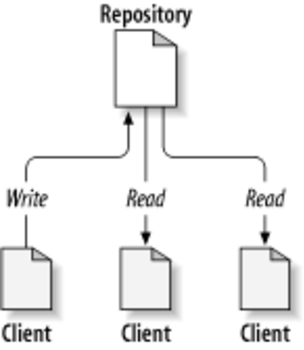
\includegraphics[width=\textwidth]{ch02dia1.pdf}
    \end{column}
  \end{columns}
\end{frame}

\begin{frame}
  \frametitle{なぜバージョン管理システムが必要なのか?}
  \begin{columns}[T]
    \begin{column}{.7\textwidth}
      \begin{itemize}
        \setlength{\itemsep}{1em}
      \item 作業者 and/or 作業場所が複数になると、ファイル名や手書きのログファイルによるバージョン管理はすぐに破綻する
        \begin{itemize}
        \item ネットワーク経由でファイルを check out/check in
        \item 更新毎に一意なバージョン番号 (リビジョン) を付与
        \item 任意のバージョン間の比較が容易
        \item バックアップの代わりにも
        \end{itemize}
      \item 複数箇所から同時に更新した場合に衝突を回避するしくみを備えている
      \item ブランチ・マージ・タグ付けなどが可能
      \end{itemize}
    \end{column}
    \begin{column}{.25\textwidth}
      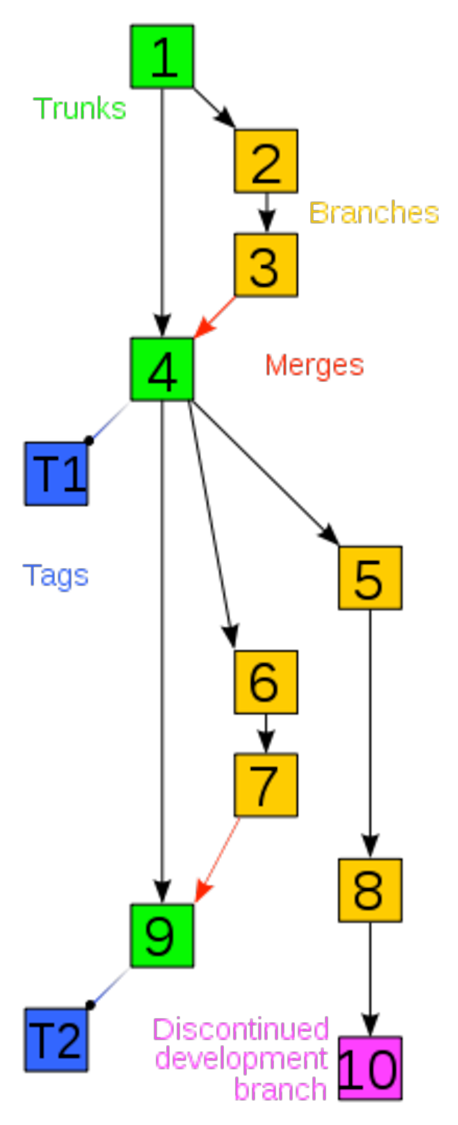
\includegraphics[width=.7\textwidth]{220px-Revision_controlled_project_visualization-2010-24-02.pdf}
    \end{column}
  \end{columns}
\end{frame}

\begin{frame}
  \frametitle{ありがちなパターン}
  \begin{center}
    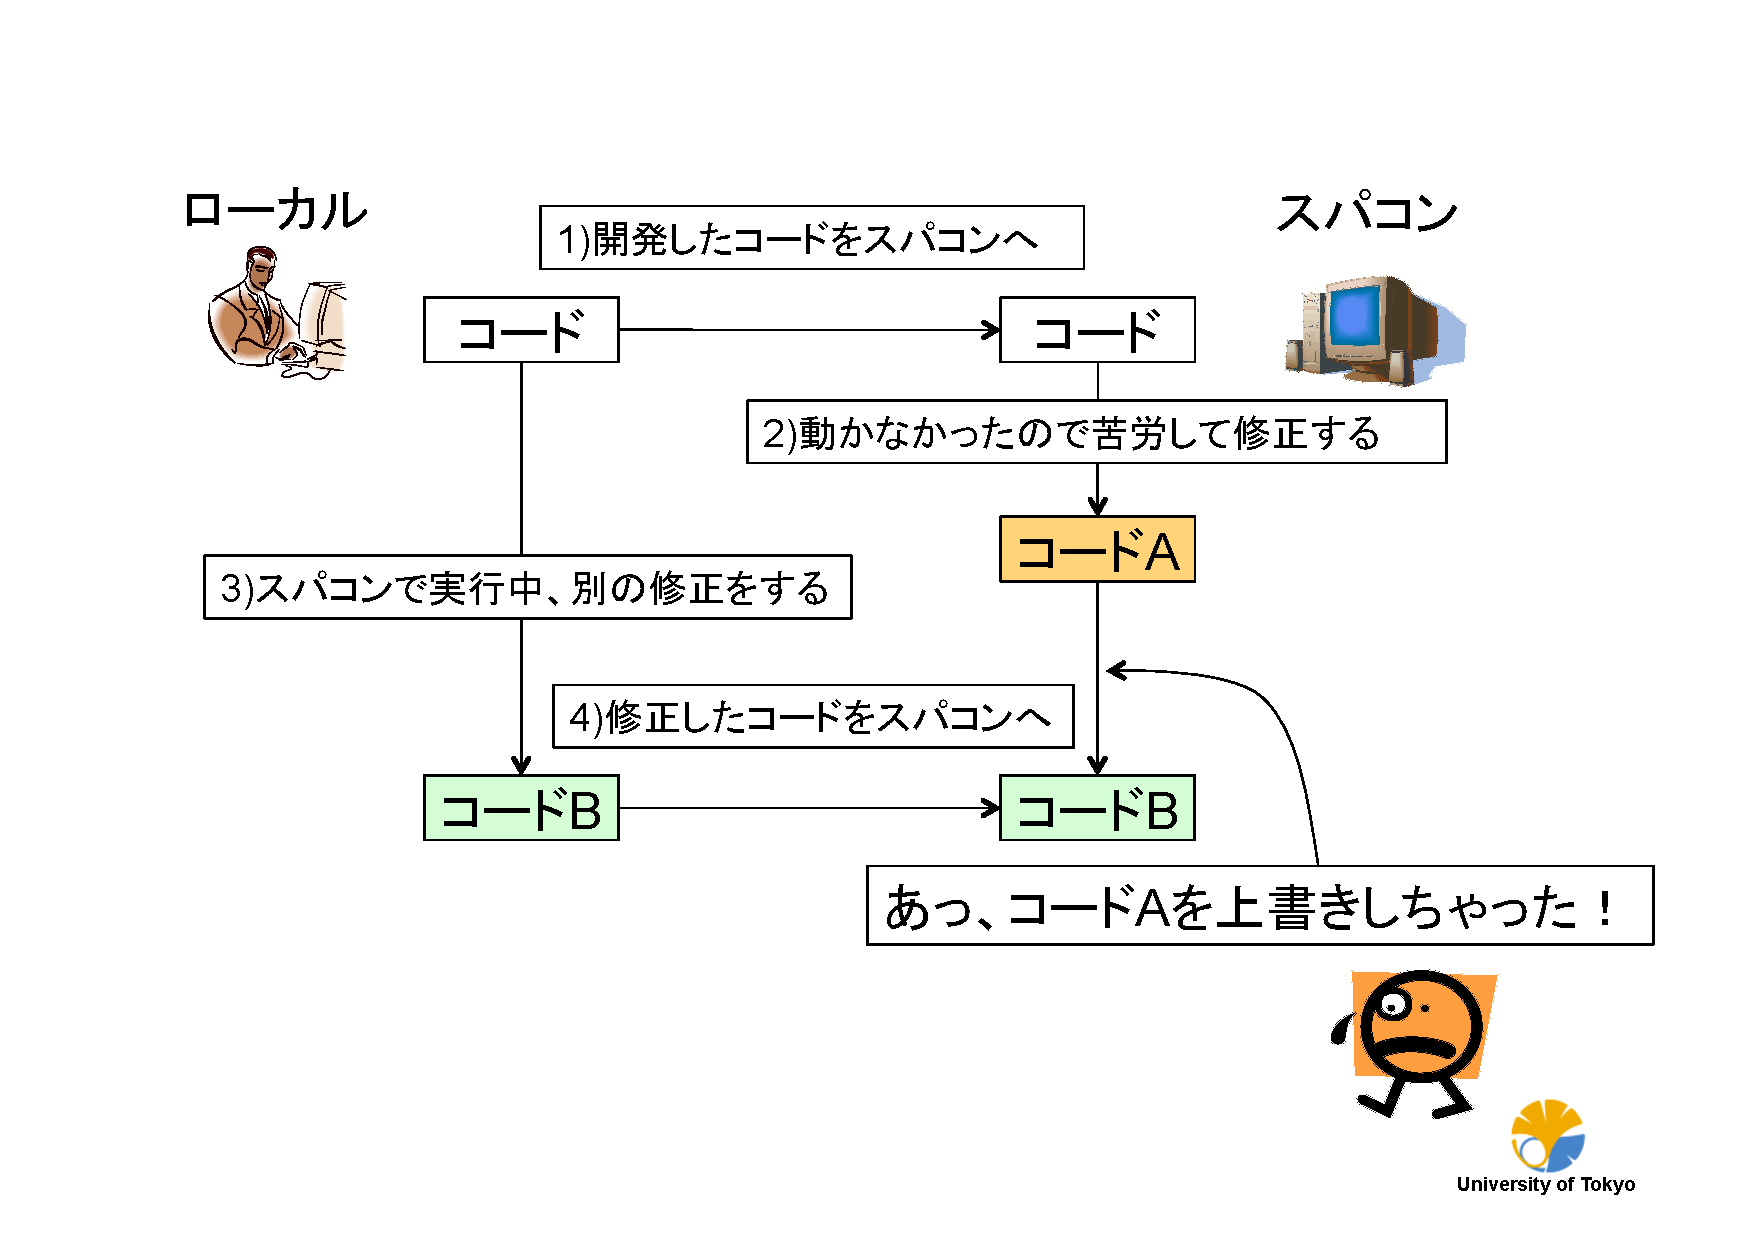
\includegraphics[height=0.88\textheight]{pattern-1.pdf}
  \end{center}
\end{frame}

\begin{frame}
  \frametitle{バージョン管理している場合}
  \begin{center}
    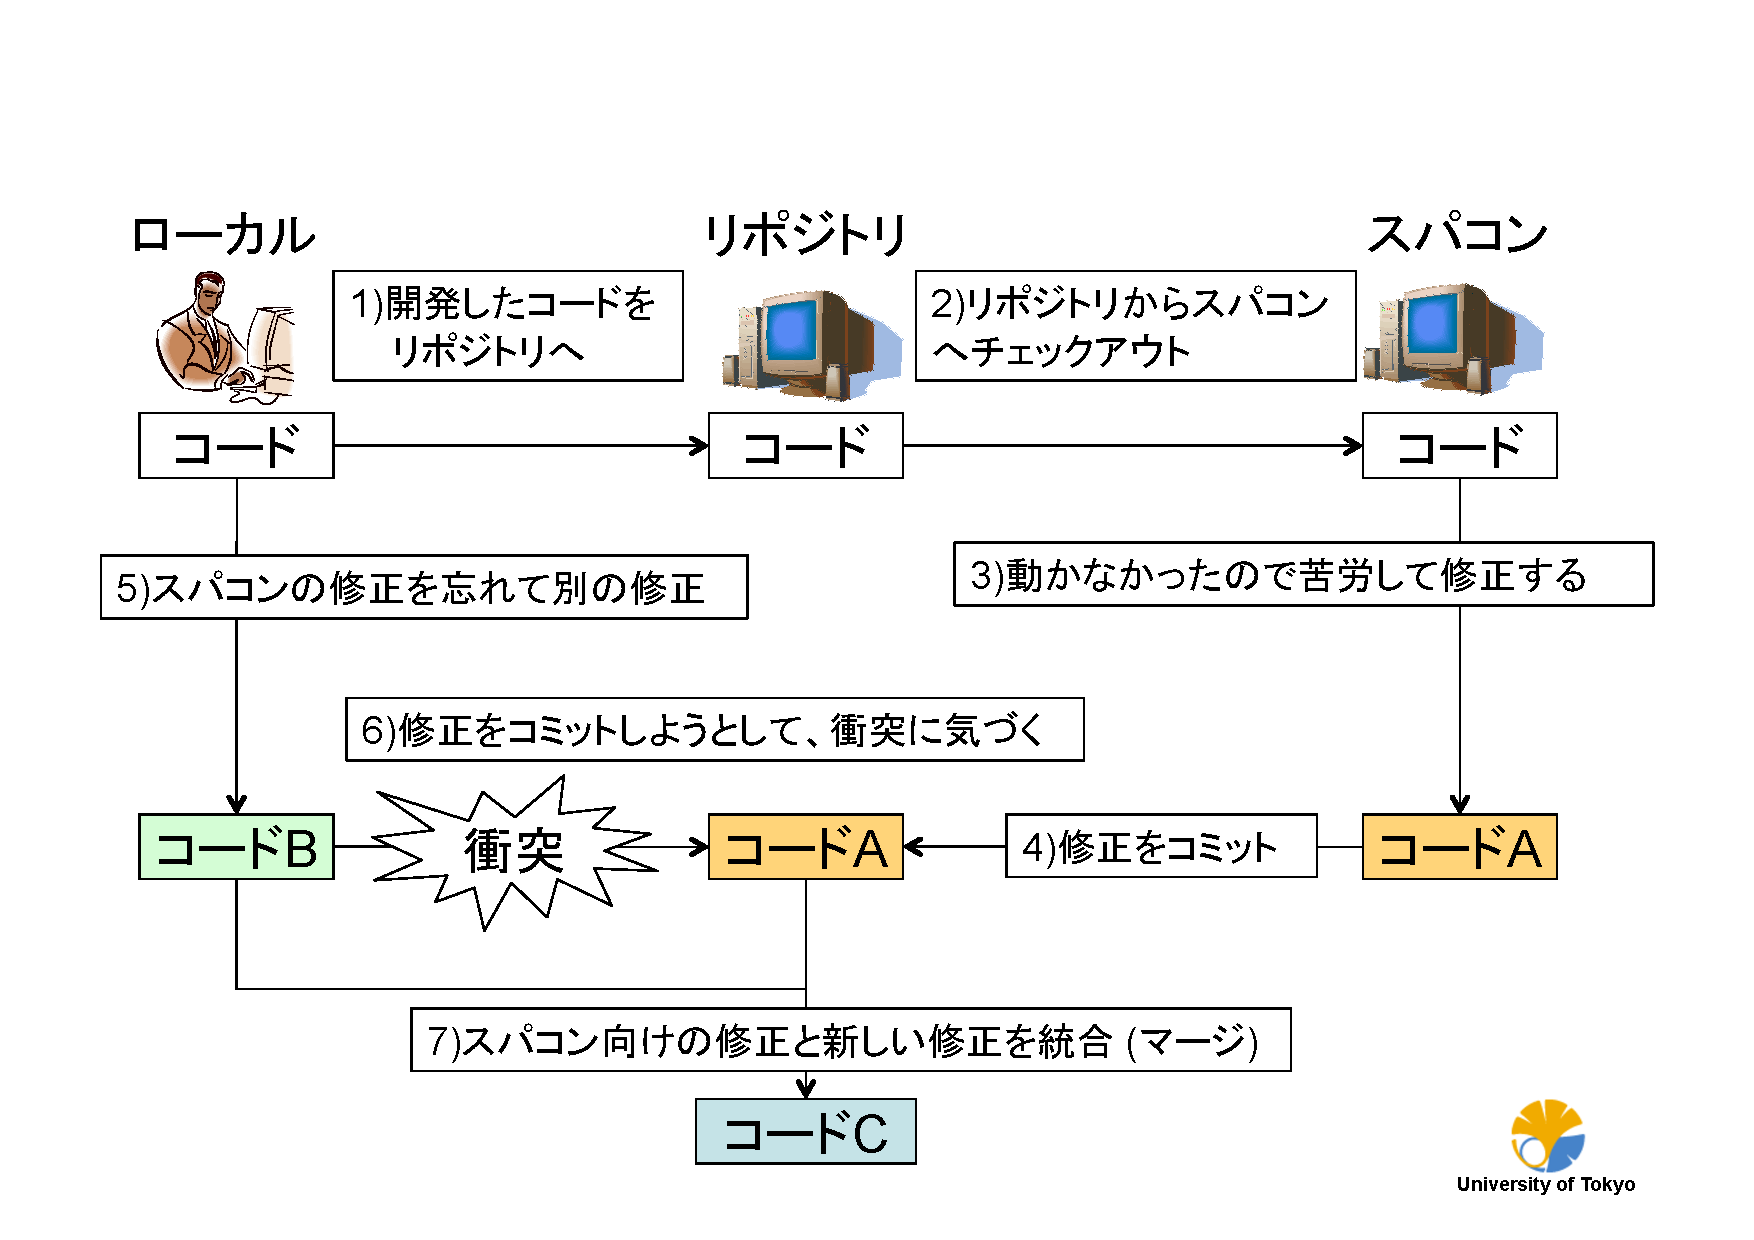
\includegraphics[height=0.88\textheight]{pattern-2.pdf}
  \end{center}
\end{frame}

\begin{frame}
  \frametitle{主なバージョン管理システム}
  \begin{itemize}
  \item BitKeeper - かつて Linux のカーネルのソース管理に使われていた
  \item CVS (Concurrent Versions System) - ネットワークでの利用を考慮とした初めてのバージョン管理システム。以前はよく使われていた
  \item Git - 現在 Linux の開発に使われている。分散型リポジトリ
  \item Mercurial - Git のライバル。分散型リポジトリ
  \item SCCS (Source Code Control System) - 70年代にベル研で開発された世界初のバージョン管理システム。現在は使われない
  \item Subversion - CVSの改良版として開発された。現在最もポピュラー? Mac OS X や多くの Linux には最初からインストールされている
  \end{itemize}
\end{frame}

\begin{frame}
  \frametitle{バージョン管理システムの欠点(面倒な点)}
  \begin{itemize}
  \item 修正前に最新の状態にアップデートしなければならない \\
   ⇒ 慣れると習慣になります
  \item 全ての修正を「コミット」しなければならない \\
    ⇒ 慣れると習慣になります
  \item 衝突(コンフリクト)が発生した時に対処しなければならない \\
    ⇒ 衝突に気づかずに修正してしまうほうが怖いです
  \item サーバのセットアップが面倒くさい \\
    ⇒ まずはホスティングサービス(sourceforge, github, bitbucket)を試してみましょう \\
    ⇒ まわりにいるプロ(?)に相談しましょう \\[.5em]
  \item バージョン管理システムを使うと作業効率が倍以上になる \\
    ⇒ {\color{red} 使わないと人生を半分損する}
  \end{itemize}
\end{frame}

\end{document}
